% Chapter 1

\chapter{Introducción general} % Main chapter title

\label{Chapter1} % For referencing the chapter elsewhere, use \ref{Chapter1} 
\label{IntroGeneral}

%----------------------------------------------------------------------------------------

% Define some commands to keep the formatting separated from the content 
\newcommand{\keyword}[1]{\textbf{#1}}
\newcommand{\tabhead}[1]{\textbf{#1}}
\newcommand{\code}[1]{\texttt{#1}}
\newcommand{\file}[1]{\texttt{\bfseries#1}}
\newcommand{\option}[1]{\texttt{\itshape#1}}
\newcommand{\grados}{$^{\circ}$}

%----------------------------------------------------------------------------------------

%\section{Introducción}

%----------------------------------------------------------------------------------------
% 1.1(5 hojas)---------------------------------------------------------------------------
%----------------------------------------------------------------------------------------
En este capítulo se presentan los conceptos básicos de la presión arterial, hipertensión y presurometrías.
Además, se menciona  el contexto y la motivación que impulsan este trabajo de investigación. 
También, se establecen los objetivos, el alcance y los requerimientos, y se revisa el estado del arte 
en el campo de estudio.

\section{Conceptos básicos de la presión arterial y sus métodos de medición}

En esta sección, se abordan las definiciones de presión arterial normal e hipertensión. 
Además, se discute el uso de las presurometrías como herramienta complementaria en el diagnóstico 
y seguimiento de paciente hipertensos.

\subsection{Presión arterial normal e hipertensión arterial}

La presión arterial (PA) es la fuerza por unidad de superficie ejercida por la sangre contra las paredes 
de las arterias \citep{CITE:1}. Sin profundizar en los principios físicos, parece relevante destacar que el corazón 
bombea la sangre de forma pulsátil. Por este motivo, la PA alterna entre una presión arterial sistólica (PAS) 
y una presión arterial diastólica (PAD). En la figura \ref{fig:aorticPulse} se expone un registro típico de las pulsaciones 
de la presión en la raíz de la arteria aorta \citep{CITE:2} \citep{CITE:3}. 

\begin{figure}[h!]
  \centering
  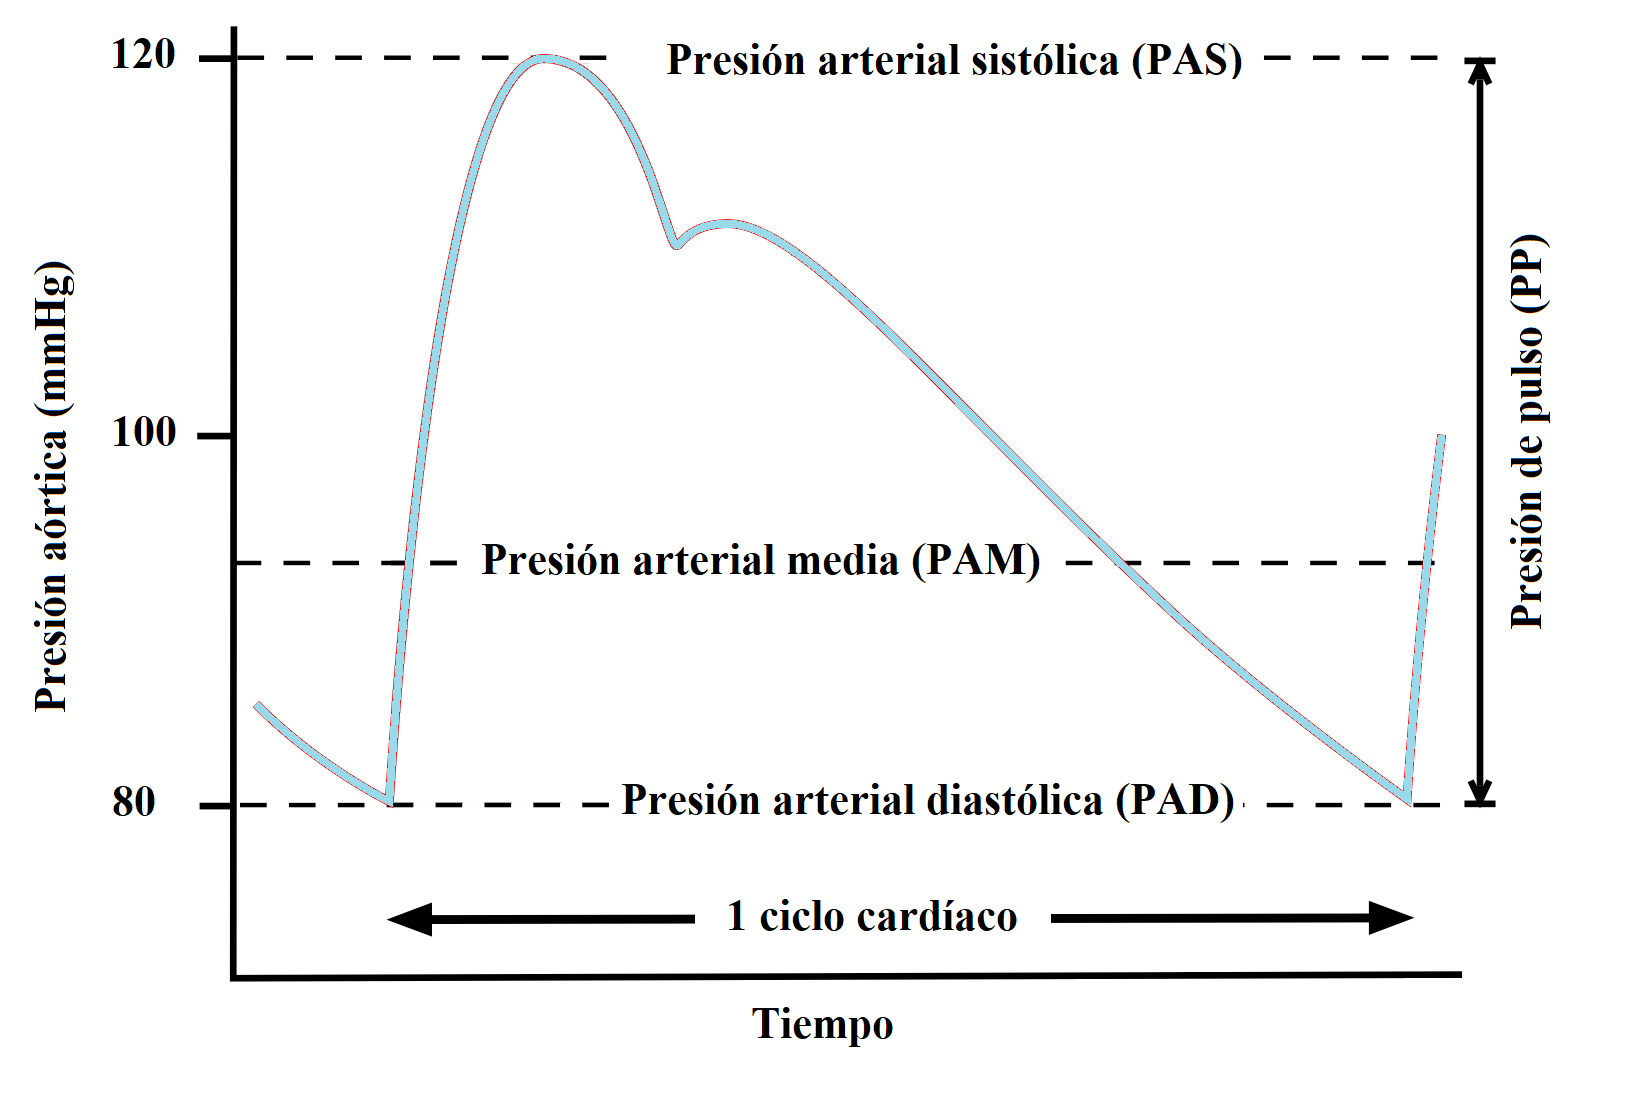
\includegraphics[width=\textwidth]{./Figures/aortic-pulse-pressure.png}
  \caption{Representación esquemática del pulso de presión registrado en la aorta ascendente\protect\footnotemark.}\label{fig:aorticPulse}
\end{figure}

\footnotetext{Imagen adaptada de Klabunde, R. E. (2013). Normal and Abnormal Blood Pressure (Physiology, Pathophysiology and Treatment). Kindle Edition.}

En un adulto joven sano, la presión máxima en cada pulso (PAS) es de 
120 mmHg y la presión mínima (PAD) es de 80 mmHg. La diferencia entre estas dos presiones 
se conoce cómo la presión de pulso (PP) y ronda unos 40 mmHg. Por otro lado, la presión arterial media (PAM) 
está determinada en un 60\% por la PAD y en un 40\% por la PAS, dado que se invierte una mayor fracción 
del ciclo cardíaco en la diástole que en la sístole \citep{CITE:2} \citep{CITE:3}. Así, la expresión matemática que describe 
a la PAM es la siguiente: 

\begin{equation}
	\label{eq:PAM}
	PAM = \frac{(2 \cdot PAD + PAS)}{3}
\end{equation}


\filbreak
% el filbreak lo puse para que el parrafo no quede cortado por el salto de pagina y la imagen de PA
La PA alta o hipertensión arterial (HTA) es uno de los principales factores de riesgo para las enfermedades 
cardiovasculares, como la enfermedad cerebrovascular, insuficiencia cardíaca, cardiopatía isquémica, 
enfermedad renal terminal, arteriopatía periférica y retinopatía. 
La HTA se clasifica en diferentes grados según los niveles de presión arterial registrados. 
De esta forma, permite evaluar y categorizar la gravedad de la HTA en los pacientes y determinar las medidas 
terapéuticas más adecuadas para su manejo \citep{CITE:6} \citep{CITE:7}. 
Actualmente, se utiliza cómo guía la clasificación de HTA de la tabla \ref{tab:TablaHTA}.

\begin{table}[h]
	\centering
	\caption[Clasificación de la presión arterial por niveles]{Clasificación de la presión arterial por niveles\protect\footnotemark.}
	\begin{tabular}{l c c c}    
		\toprule
		\textbf{Grado} 	      & \textbf{Presión arterial sistólica} 	& \textbf{}	& \textbf{Presión arterial diastólica}  \\
		\midrule
		Óptima                & <\ 120 mmHg                           & 	y			  & <\ 80 mmHg \\		
    Normal                & 120-129 mmHg                          &  	y/o			& 80-84 mmHg \\	
    Normal-alta           & 130-139 mmHg                          & 	y/o			& 85-89 mmHg \\	
    HTA de grado I        & 140-159 mmHg                          & 	y/o			& 90-99 mmHg \\
    HTA de grado II       & 160-179 mmHg                          & 	y/o			& 100-109 mmHg \\		
    HTA de grado III      & $\geq$  180 mmHg                      & 	y/o			& $\geq$  110 mmHg \\	
		\bottomrule
		\hline
	\end{tabular}
	\label{tab:TablaHTA}
\end{table}

\footnotetext{Tabla realizada con información de López Farré, A. y Macaya Miguel, C. (2009). Libro de la salud cardiovascular del hospital clínico San Carlos y la fundación BBVA (pp. 121-129). Editorial Nerea, S.A.}

\subsection{Presurometrías}

Las mediciones de la PA en el consultorio médico son necesarias pero insuficientes para un adecuado diagnóstico, 
tratamiento y seguimiento de la HTA. El monitoreo ambulatorio de presión arterial (MAPA), también conocido 
como presurometría, es un examen complementario que permite evaluar la PA en el contexto de la vida cotidiana 
del paciente. A diferencia de las mediciones de PA en el consultorio, que se realizan en condiciones 
estandarizadas, el MAPA obtiene un gran número de mediciones a lo largo de un día habitual del paciente. 
Esto proporciona la capacidad de medir la tensión arterial durante el reposo, sueño, actividad física y mental, 
trabajo y período postprandial. Conocer la PA ambulatoria permite identificar diferentes patrones de HTA, tales 
como: HTA diurna, HTA nocturna, HTA durante todo el día, HTA durante el sueño e HTA de guardapolvo blanco 
(solo presente en el consultorio médico). Por lo tanto, este estudio puede ser un predictor más efectivo de 
la mortalidad y eventos cardiovasculares que simplemente basarse en la medición de la PA en el 
consultorio médico \citep{CITE:7} \citep{CITE:5}.

Actualmente, el MAPA es el único método disponible para medir la PA durante la noche, y diversos estudios 
demuestran que la PA nocturna tiene un mayor valor pronóstico que la PA diurna. Por esta razón, se recomienda 
incluir el MAPA cómo parte del diagnóstico de la HTA. Es especialmente útil cuando los valores de PA en el 
consultorio se encuentran en un rango limítrofe (grado normal-alta según la tabla \ref{tab:TablaHTA}) en 
varias consultas consecutivas \citep{CITE:7}. Las indicaciones actuales para definir la HTA mediante el MAPA se detallan 
en la tabla \ref{tab:HTA-MAPA}.

\begin{table}[h]
	\centering
	\caption[Valores de referencia para definir HTA por MAPA]{Valores de referencia para definir HTA por MAPA\protect\footnotemark.}
	\begin{tabular}{l c c c}    
		\toprule
		\textbf{} 	      & \textbf{Presión arterial sistólica} 	& \textbf{}	& \textbf{Presión arterial diastólica}  \\
		\midrule
    PA de 24 horas     &  $\geq$ 130 mmHg                     & 	y/o			&  $\geq$ 80 mmHg \\	
    PA diurna          &  $\geq$ 135 mmHg                     & 	y/o			&  $\geq$ 85 mmHg \\	
    PA nocturna        &  $\geq$ 120 mmHg                     & 	y/o			&  $\geq$ 70 mmHg \\	
		\bottomrule
		\hline
	\end{tabular}
	\label{tab:HTA-MAPA}
\end{table}

\footnotetext{Tabla realizada con información de Cuffaro, P. E., Morales, M. S. y Waisman, G. D. (2013). MONITOREO AMBULATORIO DE PRESIÓN ARTERIAL. En SAHA (Ed.), Hipertension Arterial, Epidemiología, Fisiología, Fisiopatología, Diagnóstico y Tratamiento. (pp. 391-395). Buenos Aires.}

El MAPA se lleva a cabo mediante dispositivos conocidos como presurómetros o \textit{holters} de presión arterial. 
Un técnico en cardiología coloca el presurómetro en el brazo del paciente, y se retira al día siguiente. 
El instrumento consiste en un manguito de presión arterial conectado a una grabadora, como se muestra en 
la figura \ref{fig:holter}. Esta realiza un inflado periódico cada 20 a 30 minutos, y los datos se almacenan en una memoria 
de estado sólido, generalmente en una tarjeta SD. Luego, los datos pueden ser analizados mediante el software del 
dispositivo \citep{CITE:3} \citep{CITE:7}.

\begin{figure}[h!]
  \centering
  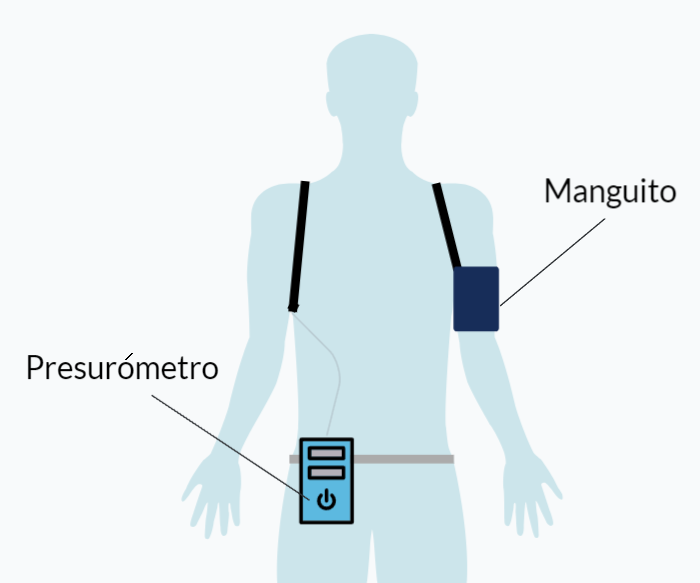
\includegraphics[width=.7\textwidth]{./Figures/presurometro.png}
  \caption{Esquema de un \textit{holter} de presión arterial.}
  \label{fig:holter}
\end{figure}


%----------------------------------------------------------------------------------------
% 1.2 (1 hoja)------------------------------------------------------------------------------------
%----------------------------------------------------------------------------------------
\newpage
\section{Contexto y motivación}

La incorporación de técnicas de inteligencia artificial (IA) en la medicina cardiovascular es una de las principales 
motivaciones en la realización de este trabajo. A medida que la IA se desarrolla en distintos campos, su aplicación 
en el ámbito de la salud experimenta un crecimiento significativo. Sin embargo, uno de los desafíos clave que la IA 
enfrenta en la medicina es la limitación de datos disponibles para entrenar modelos de aprendizaje profundo \citep{CITE:8}.

En el caso particular del Hospital Alemán de Buenos Aires, el servicio de cardiología posee una gran cantidad de 
datos de informes de presurometrías de pacientes hipertensos. Aunque el personal carece de experiencia en herramientas 
de aprendizaje automático o aprendizaje profundo, los profesionales médicos comprenden el potencial de estos datos de 
MAPA para facilitar la identificación de patrones, factores de riesgo y respuestas al tratamiento de HTA. Además, 
es importante destacar que este trabajo se alinea con la misión del Hospital Alemán, que busca la actualización constante 
de tecnologías para garantizar una mejor atención médica basada en la investigación \citep{CITE:9}. 


%----------------------------------------------------------------------------------------
% 1.3 (1 hoja)------------------------------------------------------------------------------------
%----------------------------------------------------------------------------------------

\section{Objetivos, alcance y requerimientos}

\subsection{Objetivos}
El propósito de este trabajo fue el desarrollo de un software de IA que permite predecir el riesgo de sufrir un evento 
grave en pacientes hipertensos. En particular, se busca predecir la ocurrencia de eventos cardiovasculares adversos 
mayores (MACE, por sus siglas en inglés). Este es un criterio de valoración compuesto que es empleado con frecuencia 
en la investigación cardiovascular. A pesar del uso generalizado del término en ensayos clínicos, las definiciones de 
MACE pueden diferir \citep{CITE:10}. Para este trabajo, se definió como la combinación de: accidente cerebrovascular no 
fatal, infarto agudo de miocardio, insuficiencia cardíaca, insuficiencia renal crónica o muerte. De este modo, un valor 
de MACE equivalente a la unidad indica la existencia de alguno de los eventos graves mencionados anteriormente, mientras 
que un valor nulo se refiere la ausencia de estos. 

Como resultado, este trabajo permite al servicio de cardiología e hipertensión del Hospital Alemán definir estrategias 
de tratamiento integral personalizadas para cada grupo de riesgo. 

\subsection{Alcance}
Se encuentra dentro del alcance del trabajo elaborar un dataset con variables provenientes de presurometrías. El conjunto 
de datos debe estar en cumplimiento con la ley 25.326 para garantizar el derecho al honor y a la intimidad de los 
pacientes en cuestión. Además, es parte del alcance del trabajo seleccionar y elaborar un modelo de inteligencia 
artificial que prediga MACE en pacientes hipertensos. Asimismo, se incluye en el alcance la definición de métricas 
para evaluar el correcto desempeño del modelo.

Sin embargo, no se encuentra dentro del alcance del proyecto la instalación del software desarrollado dentro de los 
establecimientos del Hospital Alemán. Tampoco se encuentra dentro del alcance la implementación de una aplicación 
visual e interactiva para que utilice el usuario final.


\subsection{Requerimientos}
A continuación, se listan los requerimientos principales del trabajo agrupados por afinidad:

\begin{enumerate}
	\item Requerimientos funcionales:
		\begin{enumerate}
			\item El código desarrollado deberá ser 
			capaz de estratificar a los pacientes en diferentes grupos de riesgo.
			\item El área bajo la curva ROC (acrónimo de \emph{Receiver Operating Characteristic}, 
			o característica operativa del receptor) del modelo deberá ser superior a 85\%.
		\end{enumerate}
	\item Requerimientos de documentación:
		\begin{enumerate}
			\item El código desarrollado deberá estar bien documentado. 
			Es decir, se deben incluir comentarios que permitan a cualquier persona comprender
			qué se está haciendo y por qué. 
		\end{enumerate}
	\item Requerimiento de testing:
		\begin{enumerate}
			\item Los resultados del código desarrollado deberán ser aprobados por el cliente 
			y los usuarios finales.
		\end{enumerate}
	\item Requerimientos reglamentarios:
		\begin{enumerate}
			\item Los datos clínicos deberán ser de carácter anónimo, cumpliendo con la ley 25.326 que reglamenta la protección de datos personales. 
			Para ello, se distinguirá a cada paciente mediante un número de identificación.
		\end{enumerate}

\end{enumerate}



%----------------------------------------------------------------------------------------
% 1.4 (1 hoja)------------------------------------------------------------------------------------
%----------------------------------------------------------------------------------------

\section{Estado del arte}

Se llevó a cabo una exhaustiva revisión de la literatura relacionada con la predicción 
de MACE a partir de datos de presurometrías.
Después de examinar la literatura, no se encontró ningún trabajo que tuviera como objetivo predecir eventos 
cardíacos mayores a partir de informes de presurometrías. Sin embargo, se hallaron trabajos que si bien no 
tienen el mismo objetivo que este, proporcionan una perspectiva útil y algunas ideas interesantes
 para el desarrollo.

En primer lugar, se encontraron trabajos que buscan predecir MACE a partir de otras fuentes, como historias clínicas 
o resultados de pruebas de laboratorio. Tal es el caso de Huang \emph{et al.} \citep{CITE:11}, Zhang \emph{et al.} \citep{CITE:12} y 
Wang \emph{et al.} \citep{CITE:13}, quienes utilizan información proveniente de historiales médicos para predecir eventos 
cardíacos mayores. Estos trabajos desarrollan modelos de aprendizaje de máquina con resultados aceptables. 
Sin embargo, es importante tener en cuenta que 
al emplear información de historiales clínicos se requiere recopilar datos durante un período prolongado. 
Esto contrasta con el uso de datos de MAPA, que brindan una visión más inmediata y detallada de la PA de los pacientes, 
permitiendo realizar inferencias en tiempo real.

En segundo lugar, existen numerosos estudios que en vez de centrarse en la predicción de MACE, se enfocan en 
predecir el riesgo de algunas enfermedades en particular. Se tuvieron en cuenta un total de 17 artículos científicos 
relevantes \citep{CITE:14} \citep{CITE:15} \citep{CITE:16} \citep{CITE:17} \citep{CITE:18}
\citep{CITE:19} \citep{CITE:20} \citep{CITE:21} \citep{CITE:22} \citep{CITE:23} \citep{CITE:24}
\citep{CITE:25} \citep{CITE:26} \citep{CITE:27} \citep{CITE:28} \citep{CITE:29} \citep{CITE:30} \citep{CITE:31}.  
Si bien los objetivos de estos estudios varían en cada caso, las técnicas de IA utilizadas son similares. 
Se puede destacar que los modelos de aprendizaje profundo demostraron el mejor rendimiento en la predicción de 
insuficiencia cardíaca y diabetes. Por otro lado, los modelos de aprendizaje de máquina clásicos obtuvieron 
los mejores resultados para la predicción de HTA.

Si bien existe literatura académica que aborda el tema de la predicción de eventos cardiovasculares, 
la mayoría de los trabajos se centran en investigaciones de carácter teórico y experimental. Sin embargo, este trabajo 
se destaca por su enfoque práctico y su objetivo de desarrollar una herramienta concreta que pueda ser implementada 
de manera efectiva en el Hospital Alemán. Mediante el uso de la presurometría  y la carga inmediata de datos, se espera 
obtener una inferencia inmediata sobre el riesgo individual de MACE. Esta iniciativa brinda una solución real y 
aplicable en el entorno clínico, mejorando así la atención y el seguimiento de los pacientes hipertensos.